\documentclass[a4paper, 12pt]{article}

\usepackage{geometry}
\geometry{left=2cm, right=2cm, top=2cm, bottom=2cm}
\usepackage{wrapfig}
\usepackage{cmap}
\usepackage{mathtext} 
\usepackage[T2A]{fontenc}
\usepackage[utf8]{inputenc}
\usepackage[english,russian]{babel}	

\usepackage{amsfonts,amssymb,amsthm,mathtools}
\usepackage{amsmath}
\usepackage{icomma} 

\usepackage{graphicx} 
\graphicspath{{picturies/}}
\usepackage{wrapfig}

\usepackage{array,tabularx,tabulary,booktabs}
\usepackage{longtable}
\usepackage{multirow}

\usepackage{caption}
\captionsetup{labelsep=period}

\renewcommand{\phi}{\varphi}
\newcommand{\eps}{\varepsilon}
\newcommand{\parag}[1]{\paragraph*{#1:}}
\newcommand{\mysec}[1]{\begin{center}\section*{#1}\end{center}}

\author{Радькин Кирилл Б01-005}
\title{3.3.5 Эффект Холла в металлах}
\date{8.10.21}

\graphicspath{{pictures/}}

\begin{document}
    \maketitle

    \parag{В работе используются} электромагнит с источником питания, источник постоянного тока, микровольтметр Ф116/1, амперметры, измеритель магнитной индукции Ш1-10, образцы из меди, серебра и цинка.

    \parag{Экспериментальная установка} Электрическая схема установки для измерения ЭДС Холла представлена на рис. 1.

    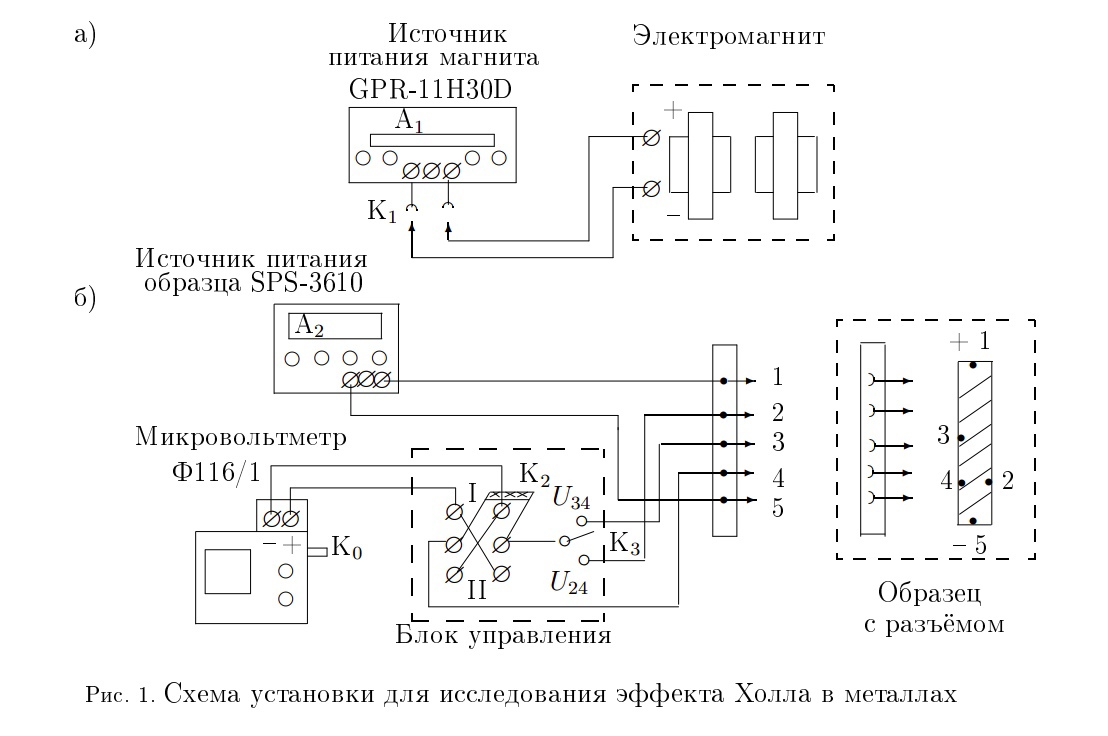
\includegraphics[width=\linewidth]{pic1.jpg}
    \\

    В зазоре электромагнита (рис. 1а) создается постоянное магнитное поле, величину которого можно менять с помощью регуляторов тока источника питания. 
    Ток питания электромагнита измеряется амперметром источника $A_1$. 
    Разъем $K_1$ позволяет менять направление тока в обмотках электромагнита. 

    Градуировка магнита проводится с помощью измерителя магнитной индукции (описание прибора расположено на установке).

    Металлические образцы в форме тонких пластинок, смонтированные в специальных держателях, подключаются к блоку питания через разъем (рис. 1б).
    Ток через образец регулируется ручками источника и измеряется амперметром источника $A_2$.

    В образце с током, помещенном в зазор электромагнита, между контактами 2 и 4 возникает холловская разность потенциалов, которая измеряется с помощью микровольтметра Ф116/1, если переключатель $K_3$ подключен к точке 2 образца.
    При подключении $K_3$ к точке 3 микровольтметр измеряет омическое падение напряжения $U_{34}$, вызванное основным током через образец.
    При нейтральном положении ключа входная цепь микровольтметра разомкнута.
    
    Ключ $K_2$ позволяет менять полярность напряжения, поступающего на вход микровольтметра.

    Иногда контакты 2 и 4 вследствие неточности  подпайки не лежат на одной эквипотенциали, и тогда напряжение между ними связано не только с эффектом Холла, но и с омическим падением напряжения, вызванным протеканием основного тока через образец.
    Измеряемая разность потенциалов при одном направлении магнитного поля равна сумме ЭДС Холла и омического падения напряжения, а при другом~---~их разности. 
    В этом случае ЭДС Холла $\eps_x$ может быть определена как половина алгебраической разности показаний вольтметра, полученных для двух противоположных направлений магнитного поля в зазоре.

    Можно исключить влияние омического падения напряжения иначе, если при каждом токе через образец измерять напряжение между точками 2 и 4 в отсутствие магнитног поля. 
    При фиксированном токе через образец это дополнительное к ЭДС Холла напряжение $U_0$ остается неизменным. 
    От него следует (с учетом знака) отсчитывать величину ЭДС Холла: $\eps_x = U_24 \pm U_0$.
    При таком способе измерения нет необходимости проводить повторные измерения с противоположным направлением магнитного поля.

    По знаку $\eps_x$ можно определить характер проводимости~---~электронный или дырочный. Для этого необходимо знать направление тока в образце и направление магнитного поля.

    Измерив ток $I$ в образце и напряжение $U_{34}$ между контактами 3 и 4 в отсутствие магнитного поля, можно, зная параметры образца, рассчитать проводимость материала образца по очевидной формуле.

    \begin{equation}
        \sigma = I  \cdot L_{34} / \left( U_{34} \cdot a \cdot l \right)
    \end{equation}
    где $L_{34}$~---~расстояние между контактами 3 и 4, $a$~---~толщина образца, $l$~---~его ширина.

    \mysec{Задание}

    В работе предлагается исследовать зависимость ЭДС Холла от величины магнитного поля при различных токах через образец для определения константы Холла; определить знак носителей заряда и проводимость различных Металлических образцов.
    Образец из серебра исследуется подробно; образец из цинка~---~по нескольким параметрам.
    \\
    \begin{center}
        Градуировка электромагнита
    \end{center}

    \begin{enumerate}
        \item С помощью прибора Ш1-10 исследуем зависимость индукции $B$ магнитного поля в зазоре электромагнита от тока через магнит.
        
        Проведем измерения магнитной индукции $B$ для 6-8 значений тока через электромагнит $I_M$ (вплоть до максимального $I_M$).

        \begin{tabular}{|c|c|c|c|c|c|c|c|c|} \hline
            $B, \text{ мТл}$ & 204 & 397 & 575 & 752 & 911 & 1009 & 1078 & 1123 \\ \hline
            $I_M, \text{ A}$ & 0.16 & 0.32 & 0.48 & 0.64 & 0.80 & 0.96 & 1.12 & 1.22 \\ \hline
        \end{tabular}
    
        \begin{center}
            Измерение ЭДС Холла
        \end{center}

        \item Вставим держатель с образцом в зазор электромагнита
        
        \item Снимем зависимость напряжения $U_{24}$ (включая $U_0$) от тока $I_M$ через обмотки магнита при фиксированном (минимальном токе) через образец. 
        Повторим  измерения при различных токах через образец. (Для напряжения~---~75 делений это 3 мкв)

        Серебряный образец:

        $U_0 = 3$ дел.

        $I_0 = 0.6 A$

        \begin{tabular}{|c|c|c|c|c|c|c|c|c|} \hline
            $U_{24}$, дел. & 6 & 7 & 10 & 12 & 15 & 16 & 17 & 19 \\ \hline
            $I_M, \text{ A}$ & 0.16 & 0.32 & 0.48 & 0.64 & 0.80 & 0.96 & 1.12 & 1.22 \\ \hline
        \end{tabular}

        $I_0 = 0.9 A$

        \begin{tabular}{|c|c|c|c|c|c|c|c|c|} \hline
            $U_{24}$, дел. & 6 & 9 & 15 & 18 & 22 & 23 & 25 & 26 \\ \hline
            $I_M, \text{ A}$ & 0.16 & 0.32 & 0.48 & 0.64 & 0.80 & 0.96 & 1.12 & 1.22 \\ \hline
        \end{tabular}

        $I_0 = 1.2 A$

        \begin{tabular}{|c|c|c|c|c|c|c|c|c|} \hline
            $U_{24}$, дел. & 8 & 14 & 19 & 23 & 28 & 30 & 32 & 33 \\ \hline
            $I_M, \text{ A}$ & 0.16 & 0.32 & 0.48 & 0.64 & 0.80 & 0.96 & 1.12 & 1.22 \\ \hline
        \end{tabular}

        Цинк:

        $U_0 = 12$ дел.

        $I_0 = 1$ A

        \begin{tabular}{|c|c|c|c|c|c|c|c|c|} \hline
            $U_{24}$, дел. & 19 & 26 & 31 & 38 & 43 & 45 & 47 & 48 \\ \hline
            $I_M, \text{ A}$ & 0.16 & 0.32 & 0.48 & 0.64 & 0.80 & 0.96 & 1.12 & 1.22 \\ \hline
        \end{tabular}

        \begin{center}
            Определение удельной проводимости
        \end{center}

        \item Выключим электромагнит
        
        \item При токе через образец $\simeq 1$ A измерим падение напряжения между контактами 3 и 4 для каждого из двух образцов. Запишем параметры образцов, указанные на держателях
        
        Цинк: $U_{34} = 480$ мкв, $L_{34} = 3.5$ мм, $a = 0.12$ мм, $l = 9$ мм

        Серебро: $U_{34} = 380$ мкв, $L_{34} = 15$ мм, $a = 0.09$ мм, $l = 11$ мм

        \item Построим график зависимости индукции магнитного поля от тока через магнит: $B = f(I_M)$
        
        \item Рассчитаем ЭДС Холла и построим на одном листе семейство характеристик $\eps_x = f(B)$ при разных значениях тока $I$ через образец (для серебра).
    
        Определим угловые коэффициенты $K(I) = \Delta \eps / \Delta B$ полученных прямых.
        
        $K1 = (6.5 \pm 0.3) \cdot 10^{-4} \text{ } \dfrac{мкВ}{мТл}$

        $K2 = (5.8 \pm 0.3) \cdot 10^{-4} \text{ } \dfrac{мкВ}{мТл}$

        $K2 = (5.4 \pm 0.2) \cdot 10^{-4} \text{ } \dfrac{мкВ}{мТл}$

        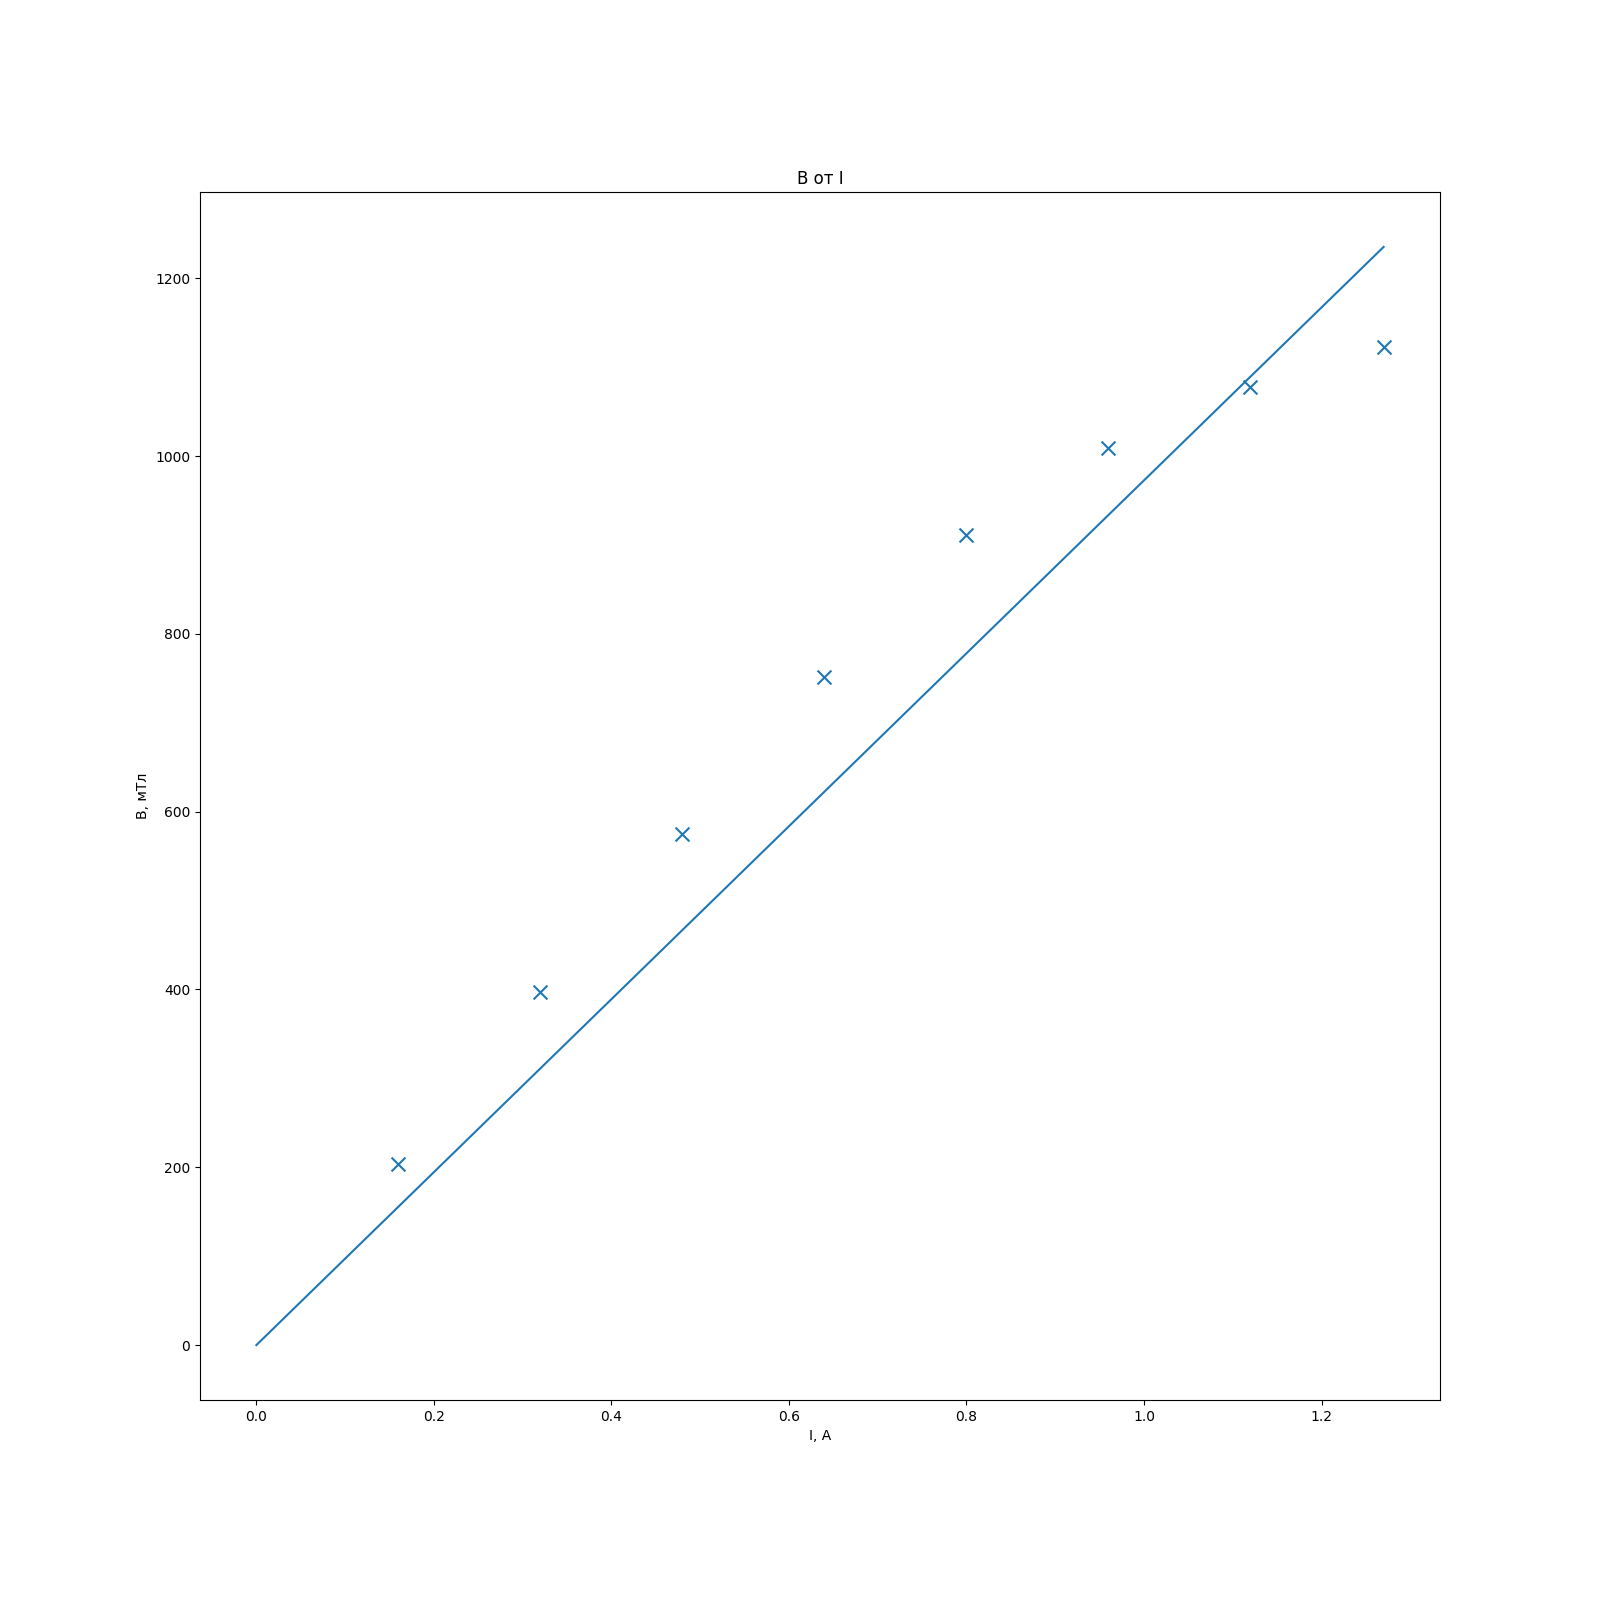
\includegraphics[scale=0.3]{graph1.png}

        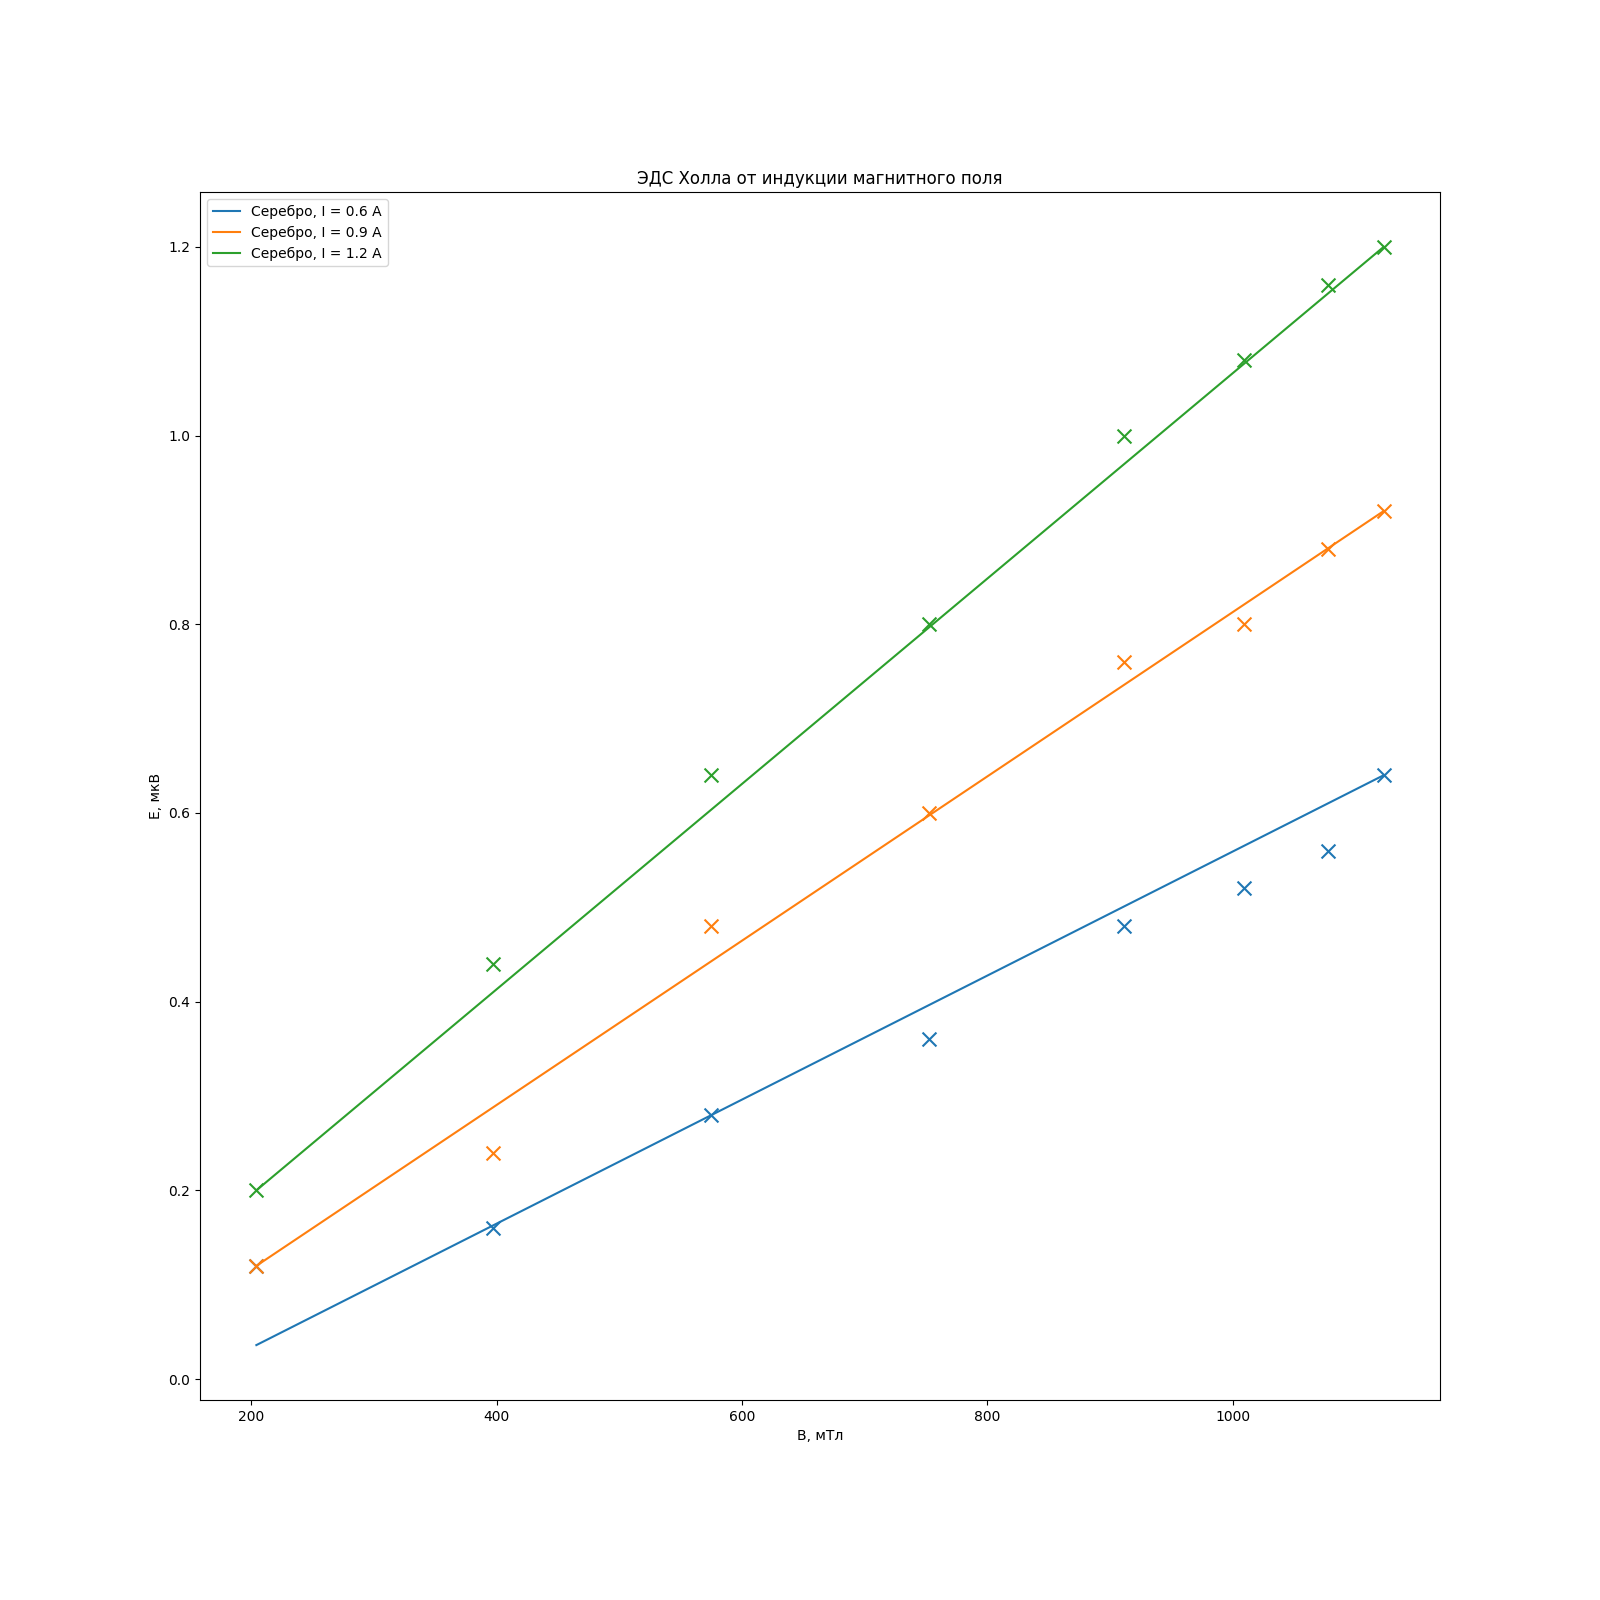
\includegraphics[scale=0.3]{graph2.png}

        \item Для цинка изобращим на графике зависимость $\eps_x = f(B)$
        
        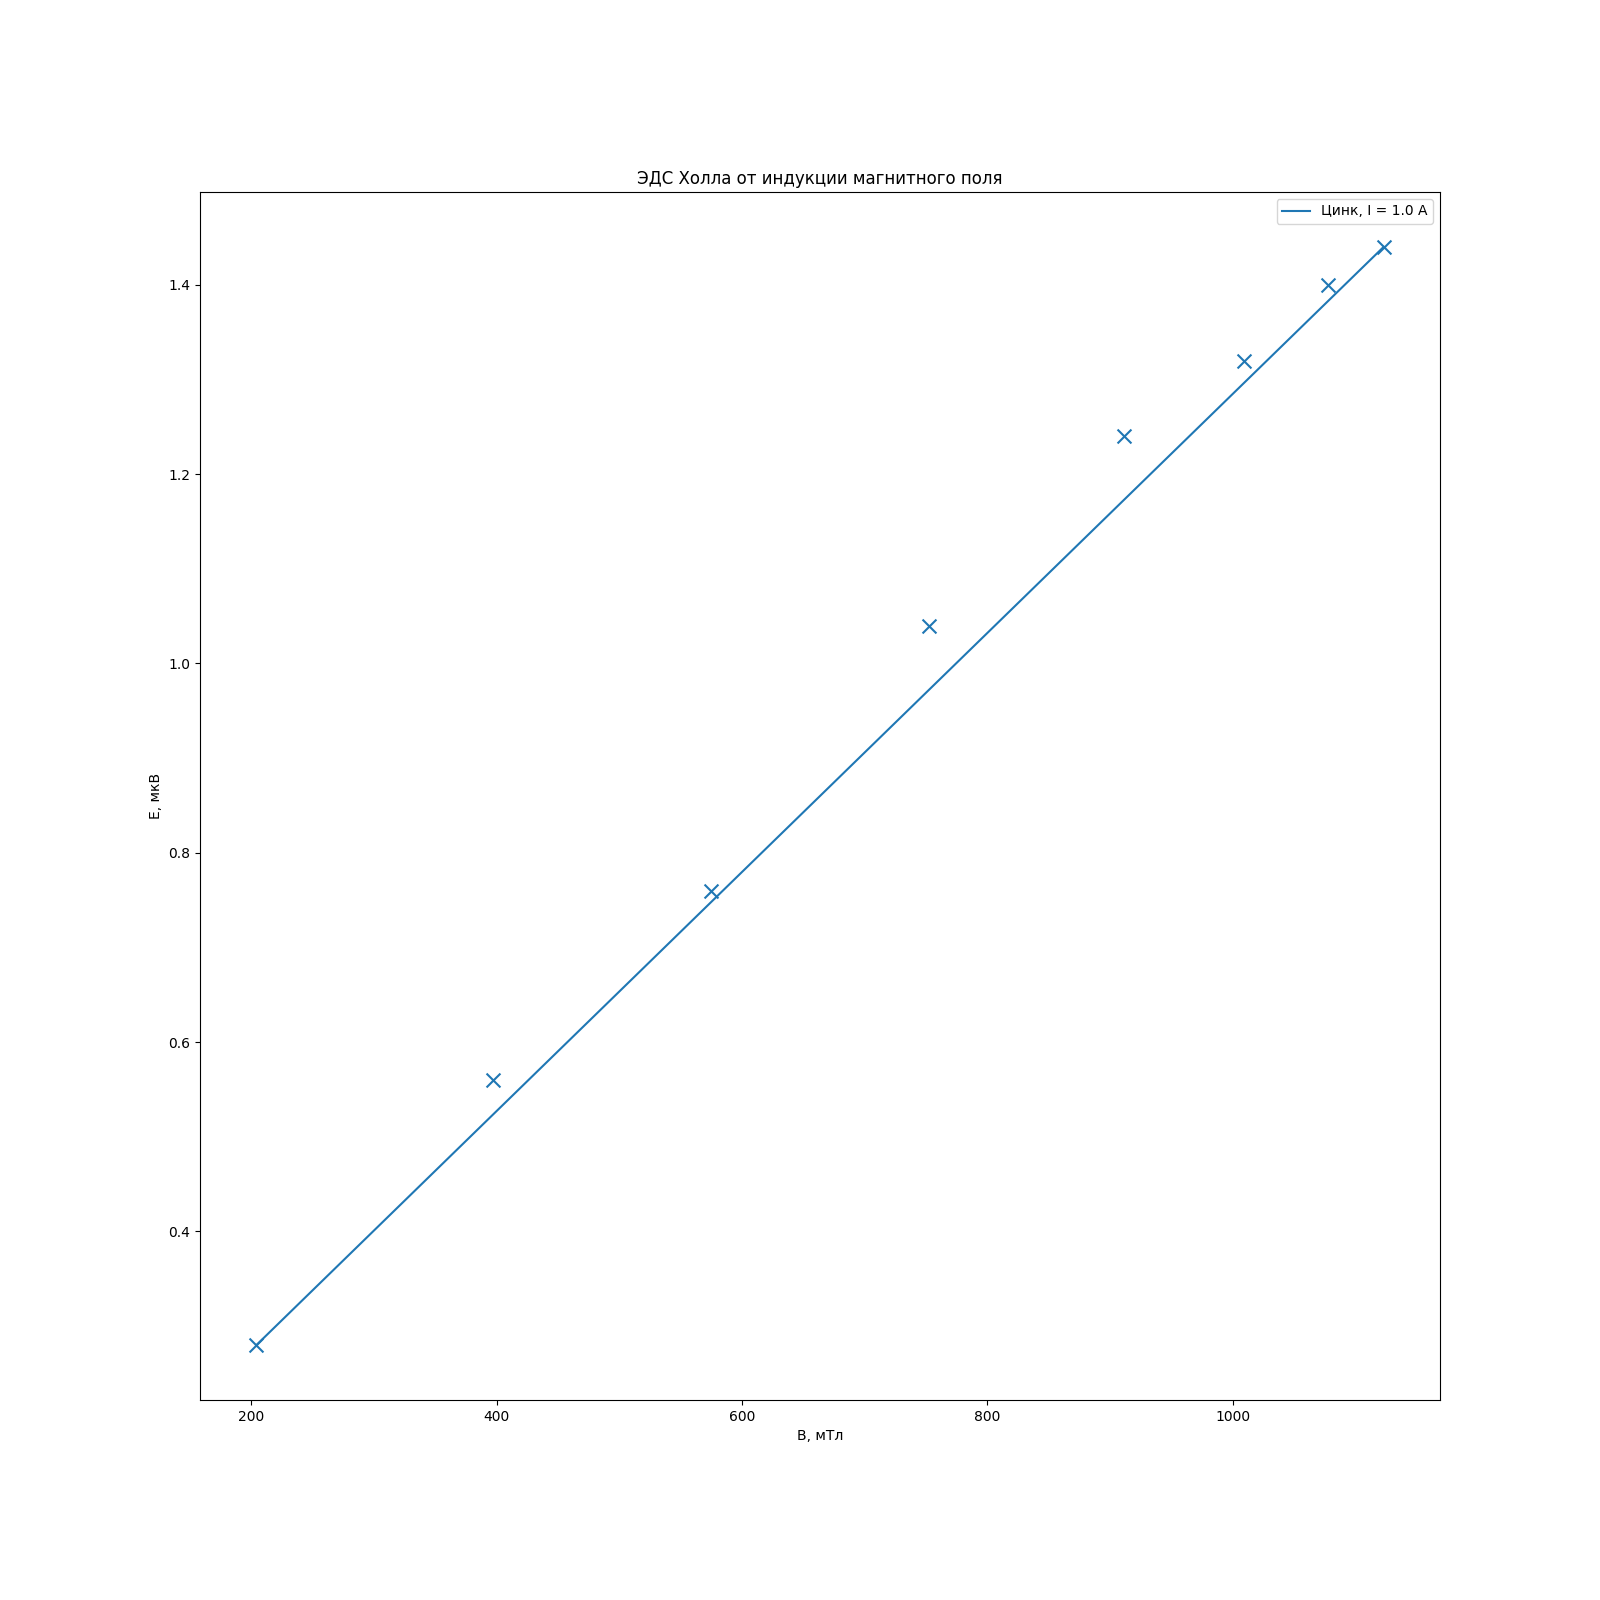
\includegraphics[scale=0.3]{graph3.png}

        \item Рассчитаем постоянные Холла для всех случаев:
        
        $R_{xs}(0.6 \text{ } A) = (9.9 \pm 0.5) \cdot 10^{-11} \text{ } \dfrac{м^3}{Кл}$

        $R_{xs}(0.9 \text{ } A) = (8.7 \pm 0.4) \cdot 10^{-11} \text{ } \dfrac{м^3}{Кл}$
        
        $R_{xs}(1.2 \text{ } A) = (8.2 \pm 0.4) \cdot 10^{-11} \text{ } \dfrac{м^3}{Кл}$

        $R_{xc}(1.0 \text{ } A) = (-15.1 \pm 1.0) \cdot 10^{-11} \text{ } \dfrac{м^3}{Кл}$

        \item Рассчитаем концентрацию $n$ носителей тока:
        
        $n_s = (15.8 \pm 1.2) \cdot 10^{30}$
        
        $n_c = (24.2 \pm 3.1) \cdot 10^{30}$

        \item Рассчитаем удельную проводимость $\sigma$ материала образцов:
        
        $\sigma_s = (39.9 \pm 4.7) \cdot 10^6 \text{ } \dfrac{1}{Ом \cdot м}$

        $\sigma_c = (6.7 \pm 0.1) \cdot 10^6 \text{ } \dfrac{1}{Ом \cdot м}$
    \end{enumerate}
   
\end{document}